\documentclass[tikz,border=10pt]{standalone}
% Scale from STYLE METRICS: s = 0.014467 cm per px, origin at circle centre O
\begin{document}
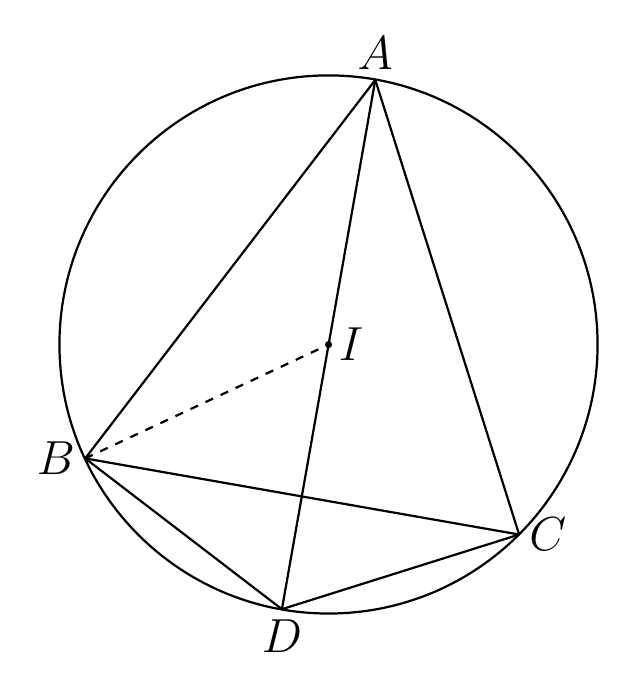
\begin{tikzpicture}[line width=0.8pt, line join=round,
    lbl/.style={font=\fontsize{17}{20.4}\selectfont}]
  % Named coordinates (cm), x=(px-283.7)*s, y=(297.3-py)*s
  \coordinate (O) at (0,0);
  \coordinate (A) at (0.594,3.360);
  \coordinate (B) at (-3.090,-1.447);
  \coordinate (C) at (2.421,-2.414);
  \coordinate (D) at (-0.592,-3.362);
  % Point I: where dashed BI meets AD (midpoint of AD, coincides with centre O)
  \coordinate (I) at (0.001,-0.001);

  % Circle (radius 236.17 px)
  \draw (O) circle (3.417);

  % Solid chords and diameter AD
  \draw (A) -- (B);
  \draw (A) -- (C);
  \draw (B) -- (C);
  \draw (B) -- (D);
  \draw (C) -- (D);
  \draw (A) -- (D);

  % Dashed segment from B to I (ends on AD)
  \draw[dashed] (B) -- (I);

  % Filled dot at I with label to its right
  \fill (I) circle (0.045);
  \node[lbl, right] at (I) {$I$};

  % Point labels outside the circle
  \node[lbl, above] at (A) {$A$};
  \node[lbl, left]  at (B) {$B$};
  \node[lbl, right] at (C) {$C$};
  \node[lbl, below] at (D) {$D$};
\end{tikzpicture}
\end{document}